\documentclass[b5paper,10pt,twoside]{book}
\usepackage[inner=1.5cm,outer=2cm,tmargin=1.5cm,bmargin=2cm]{geometry}

\usepackage[utf8]{inputenc}
\usepackage[spanish]{babel}
\usepackage{subfiles}
\usepackage{fancyhdr}
\usepackage[nottoc]{tocbibind}
\usepackage[square,numbers]{natbib}
\usepackage{titling}
\usepackage[export]{adjustbox}
\usepackage{titlesec}
\usepackage{url}
\usepackage{lipsum} 
\usepackage{graphicx}
\graphicspath{ {images/} }
\bibliographystyle{abbrvnat}
\usepackage{float}

\setcounter{secnumdepth}{3} 
\pagestyle{fancy}
\fancyhf{}
\fancyhead[LE,RO]{Diario de un superviviente}

\fancyfoot[LE,RO]{\thepage}

\title{Proyecto Fin carrera}
\author{Fernando Santa Olaya Rodríguez \\
	\and 
	Rubén Toquero González}

\date{Septiembre, 2015}
\titleformat{\chapter}[display]
{\bfseries\Large}
{\filright\MakeUppercase{\chaptertitlename} \Huge\thechapter}
{1ex}
{\titlerule\vspace{1ex}\filleft}
[\vspace{1ex}\titlerule]
\begin{document}
	
\subfile{./title}
	\chapter*{Agradecimientos}

	
	\textit{A mis padres Fernando y Filomena que me dieron a mí y a mis hermanos todo lo que ellos no tuvieron y por lo que se desvivieron trabajando, sin ellos no sería quien soy. Y a mis hermanos y hermana, David, Marta y José Ignacio, porque sin ellos mi vida hubiera sido muchísimo más aburrida y tampoco sería el hombre que hoy soy si ellos no hubiesen estado a mi lado.\\\\
		También quiero agradecer a nuestro tutor Fernando de Prada Moraga por toda la paciencia que ha tenido con nosotros, la comprensión y la ayuda que nos ha brindado tantas veces con este y otros asuntos durante la etapa estudiantil.\\\\
		A la familia más extensa, tíos, tías, primos etc por apoyarme y animarme cada vez que nos juntábamos.\\\\
		A mis amigos y compañeros de clase, la familia que eliges, por todos los sin sabores que me han acompañado a transitar en estos años y no mandarme muy lejos casi nunca.\\\\
		A Rubén por ser mi motor en esta última etapa y forzarme a empujar un poco más cada día y robar tiempo de donde no lo había.\\\\
		Por último a todos aquellos profesores que me ayudaron a llegar aquí, desde EGB hasta este último proyecto, por saber despertar la curiosidad y ansia de saber y por su dedicación a mi formación no sólo como ingeniero sino también como persona.\\
		Fernando Santa Olaya Rodríguez\\\\\\
		Quiero agradecer a mi familia todo el apoyo que me han dado durante todos estos años, a los que están y a los que ya no están, a los que dedico este trabajo por razones obvias.\\\\
		También quiero agradecer al tutor Fernando de Prada Moraga toda la paciencia que ha tenido con nosotros, nos ha comprendido y nos ha ayudado a llevar a cabo esta necesaria tarea.\\\\
		A Nuria, que es la que me ha sufrido la mayor parte del tiempo, todavía me resulta incomprensible que me siga aguantando después de tantos años.\\\\
		A Fer que también me ha aguantado como un jabato y ha tenido paciencia y comprensión.\\\\
		Por último agradezco a los profesores de esta escuela sus enseñanzas (espero que bien aprovechadas por mi parte) y a todos aquellos con los que he compartido mi tiempo en mi paso por esta etapa de la vida que aquí se cierra, o no.\\*
		Rubén Toquero González} 
	

	\chapter*{Resumen}
		El presente proyecto implementa una aplicación móvil enmarcada dentro del programa 'Diario de salud para supervivientes de Cáncer' de la Asociación Española Contra el Cáncer (AECC), esta aplicación funcionará como un micro asistente virtual para personas que padezcan o hayan padecido la lacra moderna que resulta ser la enfermedad del cáncer.\\*
		
		Es decir, esta aplicación proporcionará las herramientas necesarias para llevar al día el control de los cuidados necesarios para el tratamiento de un paciente que ha superado la enfermedad pero necesita llevar un control de sus actividades rutinarias, citas médicas, medicación, pruebas, síntomas y de las personas que participan diariamente de su vida.\\*
		
		Esta aplicación es la evolución lógica del libro que utiliza la AECC para guiar a los 'supervivientes' de la enfermedad a enfocar su día a día y facilitarles la convivencia con las acciones dedicadas o no al tratamiento de su enfermedad y a hacer de este algo más llevadero.\\*
		
		El presente proyecto implementa una aplicación móvil como micro asistente virtual para personas que padezcan o hayan padecido la lacra moderna del cáncer y una aplicación en servidor con la que se comunica la app y recopila estadísticas de actividades y estados de animo de los usuarios para su posibles estudios relacionados con la enfermedad. Ademas provee de una plataforma con la que se puede interactuar fácilmente con los usuarios de la misma por un operador de la misma. Todo esto se incluye dentro de la iniciativa "Diario de un superviviente" de la Asociación Española contra el Cáncer.\\*
	 	
	\begin{figure}[h]
		\centering
		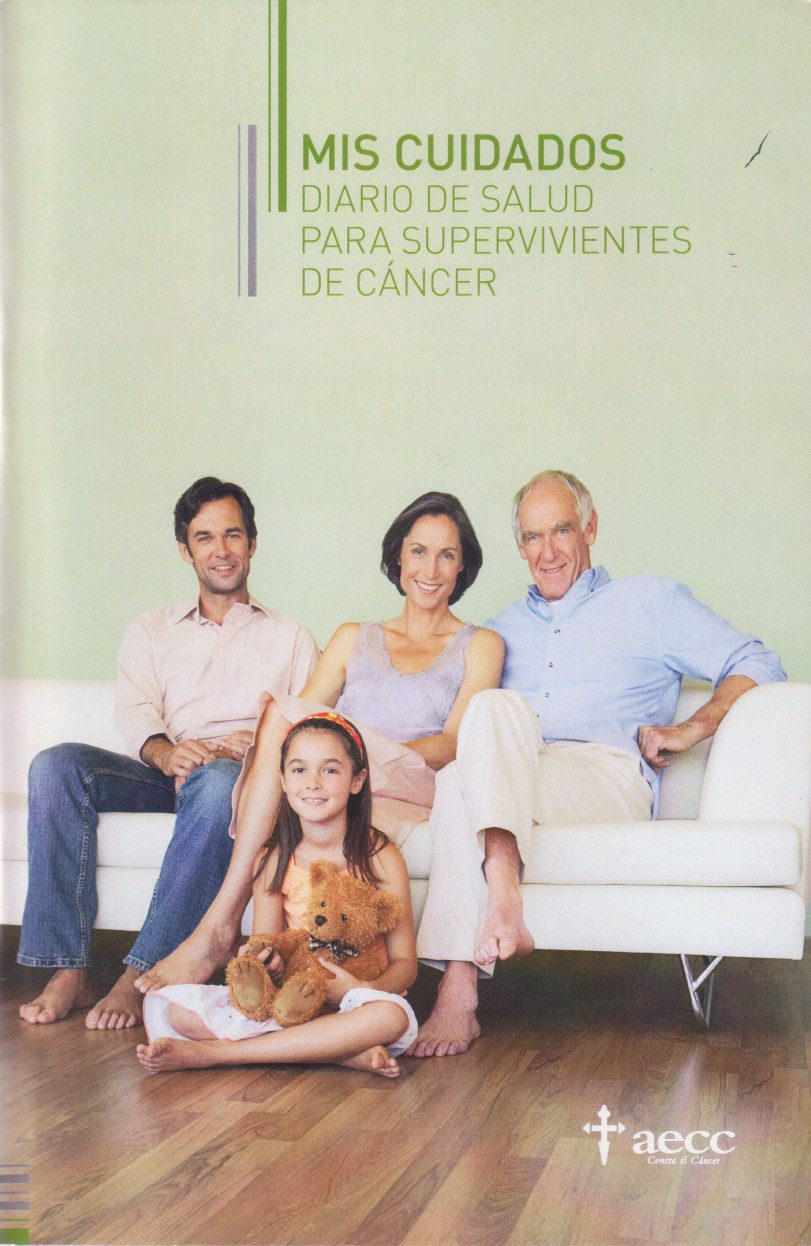
\includegraphics[width=0.25\textwidth]{fotointro}
		\caption{Portada del folleto de la AECC.}
		\label{fig:mesh1}
	\end{figure}
	 
	\chapter*{Abstract}
	 	This project implements a mobile application as micro virtual assistant to people suffering from the modern scourge of cancer and an application server with the app communicates and gathers statistics activities and moods of users for possible studies related to the disease. Also provides a platform that can easily interact with users of the same for the same operator. All this is included in the "Diary of a Survivor" initiative of the Spanish Association Against Cancer. This project implements a mobile application as micro virtual assistant to people suffering from the modern scourge of cancer and an application server with the app communicates and gathers statistics activities and moods of users for possible studies related to the disease. Also provides a platform that can easily interact with users of the same for the same operator. All this is included in the "Diary of a Survivor" initiative of the Spanish Association Against Cancer.\cite{SHAREESP}
	
	\tableofcontents
	
	\listoffigures
	
	\listoftables
	

	\chapter{Introducción}
	
	\subfile{./1-Introduccion/introduccion}
	
	\chapter{Visión general del Proyecto}

	\subfile{./2-Vision/vision}
	
	\chapter{Planificación y Metodología}
	
	\subfile{./3-Planificacion/planificacion}
	
	\chapter{Análisis}
	
	\subfile{./4-Analisis/analisis}
	
	\chapter{Diseño}
	
	\subfile{./5-Diseno/diseno}
	
	\chapter{Implementación y Pruebas}
	
	\subfile{./6-Pruebas/pruebas}
	
	\chapter{Conclusiones y trabajo futuro}
	
	\subfile{./7-Conclusiones/conclusiones}
	
	\chapter{Bibliografía}
	
	\bibliography{bibliography}
	
	\chapter*{ANEXO I: INSTALACIÓN Y MANUAL DE USUARIO }
		
	\subfile{./8-Anexoi/anexoi}
	
	\chapter*{GLOSARIO}
	
	\subfile{./Glosario/glosario}

\end{document} 